\documentclass[12pt]{article}

% PACKAGES

\usepackage[
top=2.50cm,
bottom=2.50cm,
left=2cm,
right=2cm,
marginparsep=0pt,
marginparwidth=0pt]{geometry}
\usepackage{fancyhdr}
\usepackage{float}
\usepackage{dirtree}
\usepackage{cancel}
\usepackage{mathtools}
\usepackage{amsmath}
\usepackage{amsthm}
\usepackage{amssymb}
\usepackage{textcomp}
\usepackage{ulem}
\usepackage{verbatim}
\usepackage{contour}
\usepackage{graphicx}
\usepackage{svg}
\usepackage{xcolor}
\usepackage[T1]{fontenc}
\usepackage{inputenc}
\usepackage[utf8]{inputenx}
\usepackage[unicode]{hyperref}
\usepackage[shortlabels]{enumitem}
\usepackage{booktabs}
\usepackage{bookmark}
\usepackage{listings}
\usepackage{xcolor}
\usepackage{tocloft}
\usepackage{tikz}
\usepackage[backend=biber]{biblatex}

% MACROS & DEFS

\newcommand{\floor}[1]{\left\lfloor #1 \right\rfloor}
\newcommand{\ceil}[1]{\left\lceil #1 \right\rceil}
\newcommand{\round}[1]{\left\lfloor #1 \right\rceil}
\newcommand{\abs}[1]{\left\lvert #1 \right\rvert}

\DeclareRobustCommand{\ul}[1]{%
	\uline{\phantom{#1}}%
	\llap{\contour{white}{#1}}%
}

\renewcommand{\ULdepth}{1.8pt}
\contourlength{0.8pt}

\setlength{\parindent}{0em}
\setlength{\parskip}{0.75em}

\definecolor{codegreen}{RGB}{0,135,0}
\definecolor{codegray}{RGB}{135,135,135}
\definecolor{codemagenta}{RGB}{215,0,135}
\definecolor{codepurple}{RGB}{135,0,175}
\definecolor{backcolour}{RGB}{238,238,238}

% PACKAGE CONFIG

\graphicspath{ {./images/} }

\lstdefinestyle{code}{
	basicstyle=\ttfamily\small,
	commentstyle=\color{codegray}\itshape,
	keywordstyle=\color{codepurple},
	stringstyle=\color{codegreen},
	aboveskip=25pt,
  belowskip=10pt,
	captionpos=b,
	abovecaptionskip=12.5pt,
	breaklines=true,
	numbers=none,
	frame=tb,
	framesep=5pt,
	keepspaces=true,
	showspaces=false,
	showstringspaces=false,
	breakatwhitespace=false,
	tabsize=2,
	showtabs=false,
}

\lstset{style=code}

% Set dots for table of contents
\renewcommand{\cftdot}{.}
\renewcommand{\cftsecleader}{\cftdotfill{\cftdotsep}}

% Set theorem
\newtheorem*{definition}{Definition}

% HEADER & FOOTER

\setlength{\headheight}{15pt}
\pagestyle{fancy}
\renewcommand{\headrulewidth}{0pt}
\lhead{J. Scerri}
\chead{CPS1012 --- Coursework}
\rhead{\thepage}

% TITLE

\title{CPS1012 --- Operating Systems \& Systems Programming 1\\
\vspace{1em}\textbf{Coursework}}

\date{\today}

\author {{\textbf{Juan Scerri}}\\
B.Sc. (Hons)(Melit.) Computing Science and Mathematics (First Year)}

\begin{document}

%----------------------------------
%	TITLE PAGE
%----------------------------------

\maketitle % Print the title page

\thispagestyle{empty} % Suppress headers and footers on the title page

%----------------------------------

\tableofcontents

\clearpage

\listoffigures

\lstlistoflistings

\clearpage

\section{Plagiarism Declaration}

Plagiarism is defined as \textit{``the unacknowledged use, as
one's own, of work of another person, whether or not such work
has been published, and as may be further elaborated in Faculty
or University guidelines''} (\ul{University Assessment
Regulations}, 2009, Regulation 39 (b)(i), University of Malta).

I, the undersigned, declare that the report submitted is my
work, except where acknowledged and referenced. I understand
that the penalties for committing a breach of the regulations
include loss of marks; cancellation of examination results;
enforced suspension of studies; or expulsion from the degree
programme.

Work submitted without this signed declaration will not be
corrected, and will be given zero marks.

\vfill

\begin{minipage}[t]{0.3\textwidth}
\ul{Juan Scerri} \medskip

\textbf{Student's full name} \medskip
\end{minipage}
\hfill
\begin{minipage}[t]{0.3\textwidth}
\ul{CPS1012} \medskip

\textbf{Study-unit code} \medskip
\end{minipage}
\hfill
\begin{minipage}[t]{0.3\textwidth}
\ul{{\today}} \medskip

\textbf{Date of submission} \medskip
\end{minipage}

\vspace{2cm}

\textbf{Title of submitted work:} \ul{Operating Systems \&
Systems Programming 1 Coursework}

\vspace{2cm}

\textbf{Student's signature} \medskip

\underline{
\includegraphics[height=2cm]{sig}} \medskip

\section{Structure \& Design}

\subsection{Structure}

The coursework was broken up into four tasks.

All the questions from \textit{Task 1} have been answered
separately, each having there own \texttt{.c} file.

The two questions from \textit{Task 2} were answered in one
\texttt{.c} file.

\textit{Task 3} and \textit{Task 4} were done simultaneously to
avoid code repetition and reduce complexity of development. This
is because it is easier to develop an interpreter where all the
constraints are known.

Naturally, some of the code developed for \textit{Task 1} and
\textit{Task 2} was copied over to the directory of \textit{Task
3} and \textit{Task 4}. Specifically, the relevant code from
\textit{Task 1} was placed in \texttt{external.c} and the
relevant code from \textit{Task 2} was placed in
\texttt{builtin.c}.

\textit{Note:} There is an extra directory called \texttt{util}
which contains older versions of code which can be found in
\texttt{interpreter.c}. The header files within this directory
are used in \textit{Task 1} and \textit{Task 2} to allow for
easier testing.

\begin{center}
\begin{minipage}[t]{0.3\textwidth}
\dirtree{%
.1 /.
.2 src.
.3 task1.
.3 task2.
.3 task3and4.
.3 util.
.3 .clang-format.
.3 CMakeLists.txt.
.2 .clang-format.
.2 .gitignore.
.2 README.md.
}
\end{minipage}
\begin{minipage}[t]{0.3\textwidth}
\dirtree{%
.1 util.
.2 .clang-format.
.2 linenoise.c.
.2 linenoise.h.
.2 peek\_stream.c.
.2 peek\_stream.h.
.2 string\_vec.c.
.2 string\_vec.h.
.2 tokeniser.c.
.2 tokeniser.h.
.2 util.h.
}
\end{minipage}
\end{center}

\begin{center}
\begin{minipage}[t]{0.3\textwidth}
\dirtree{%
.1 task1.
.2 .clang-format.
.2 qa.c.
.2 qb.c.
.2 qc.c.
.2 qd.c.
.2 qe.c.
}
\end{minipage}
\begin{minipage}[t]{0.3\textwidth}
\dirtree{%
.1 task2.
.2 .clang-format.
.2 qab.c.
}
\end{minipage}
\begin{minipage}[t]{0.3\textwidth}
\dirtree{%
.1 task3and4.
.2 .clang-format.
.2 builtin.c.
.2 builtin.h.
.2 external.c.
.2 external.h.
.2 interpreter.c.
.2 interpreter.h.
.2 linenoise.c.
.2 linenoise.h.
.2 tests.txt.
.2 tish.c.
}
\end{minipage}
\end{center}

\subsection{Design}

In this section the majority of the design will be explained
through illustrations. Where necessary supplementary explanation
will be provided and code snippets will be inserted.

\subsubsection{Design of Task 1}

\begin{figure}[H]
\centering
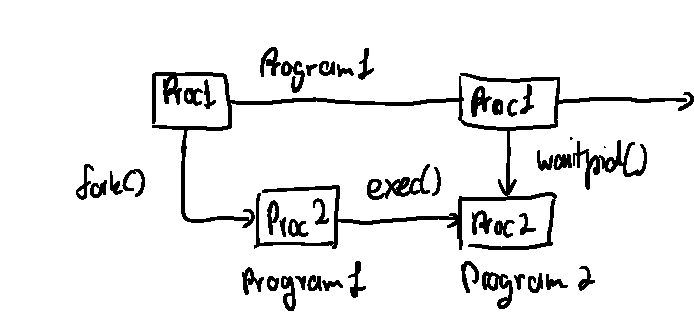
\includegraphics[height=4.5cm]{task1qa}
\caption{An illustration of the \texttt{fork-exec-wait} pattern.}
\end{figure}

\lstinputlisting[caption={An implementation of the
\texttt{fork-exec-wait} pattern.},language=C, firstline=24,
lastline=34]{src/task1/qa.c}

For question (a), the requested algorithm implements a simple
\texttt{fork-exec-wait} pattern. This pattern is used to allow
processes to load other programs.

\begin{figure}[H]
\centering
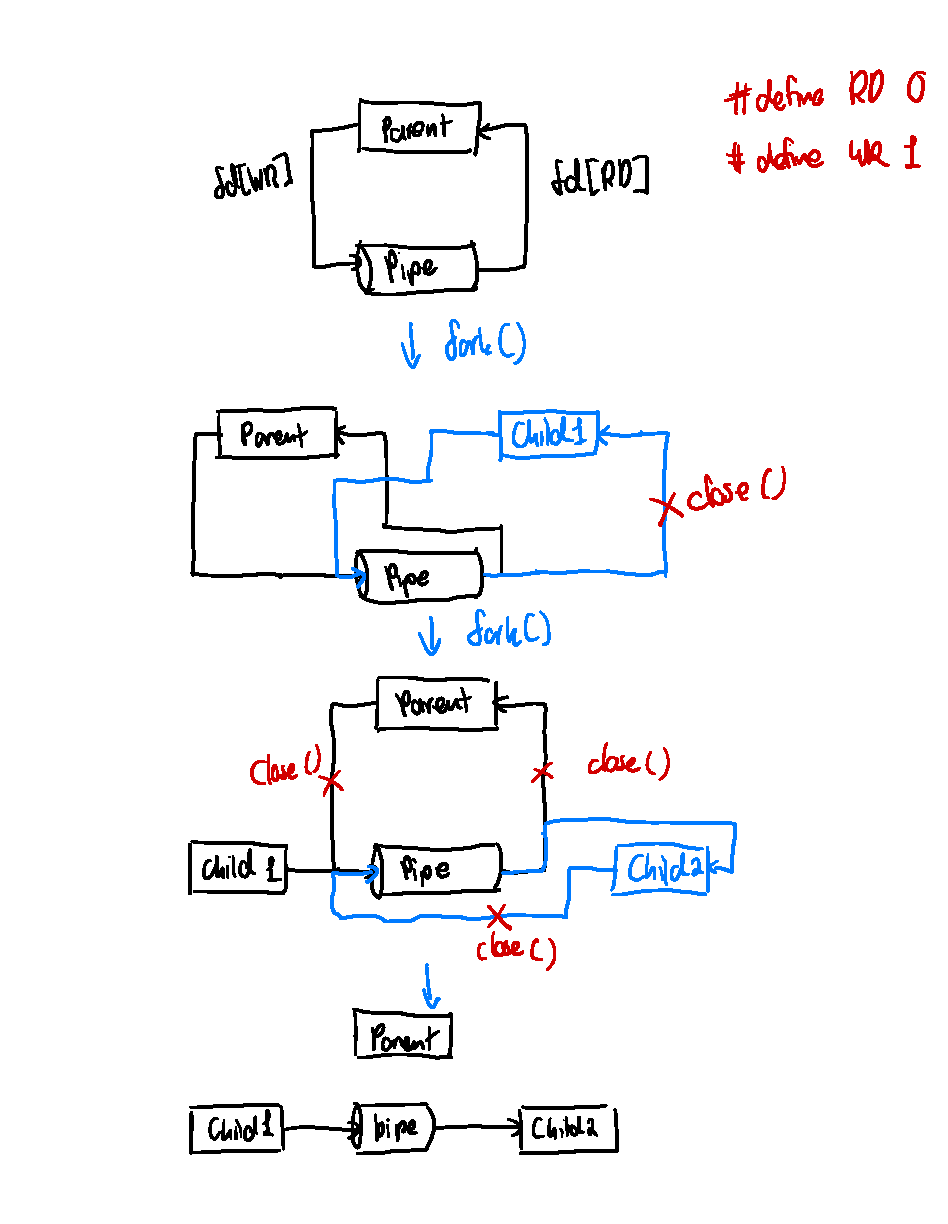
\includegraphics{task1qb}
\caption{An illustration of the pattern used to connect two
processes through a pipe.}
\label{create_pipe}
\end{figure}

\newpage

The pattern described in \ref{create_pipe} is used to allow two
processes to communicate with each other. This communication is
facilitated by a pipe. Pipes are an Inter-Process
Communication (IPC) mechanism provided by the OS.

\lstinputlisting[caption={Configuration of a pipe after
\texttt{fork()} and before \texttt{execvp()}.},language=C,
firstline=37, lastline=47]{src/task1/qb.c}

\textit{Note:} Configuration of the pipes is done after
\texttt{fork()} and before \texttt{execvp()} (or any other
variant of \texttt{exec()}).

\begin{figure}[H]
\centering
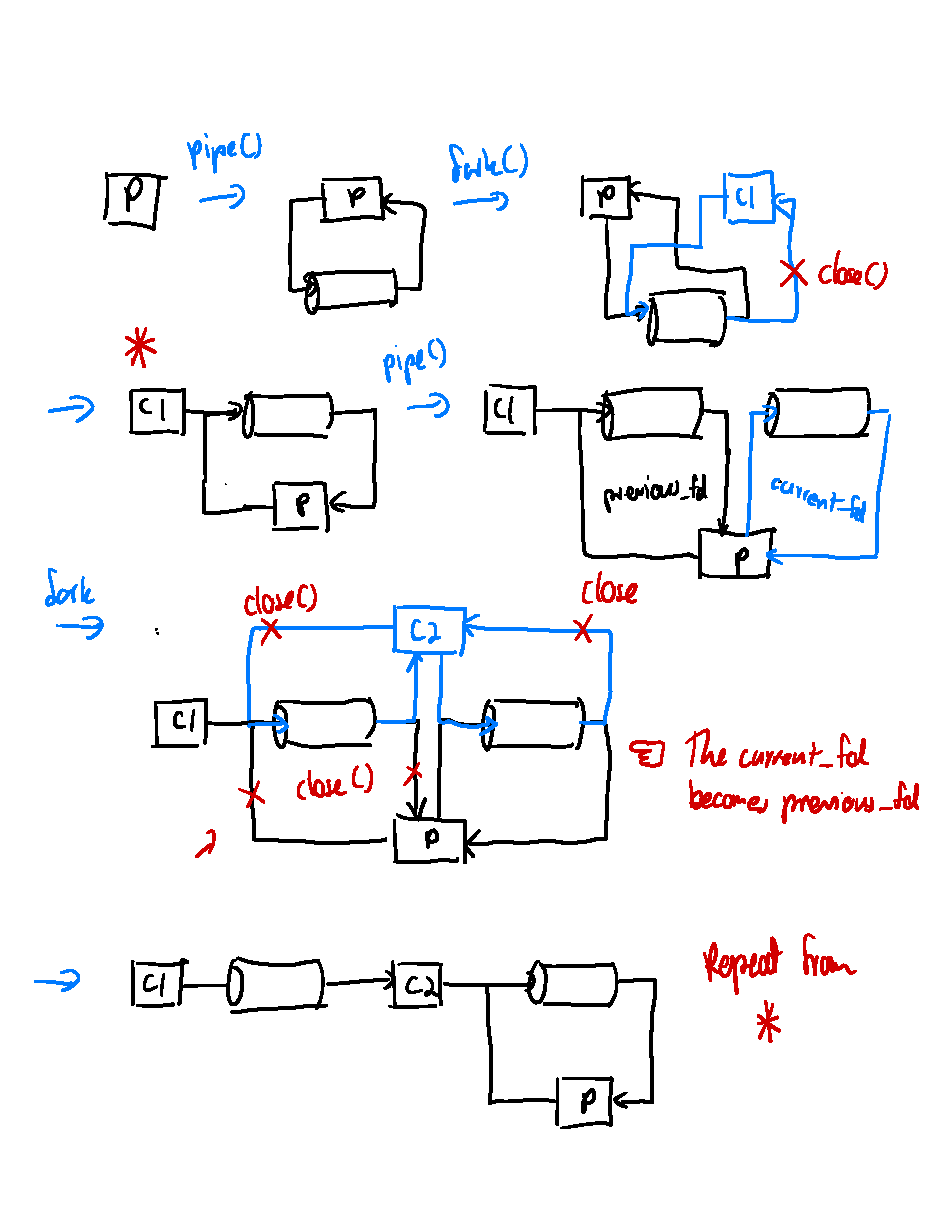
\includegraphics{task1qc1}
\caption{An illustration of the \ul{start} and \ul{middle}
patterns used to construct an arbitrary pipeline.}
\label{gen_pipeline}
\end{figure}

\newpage

\begin{figure}[H]
\centering
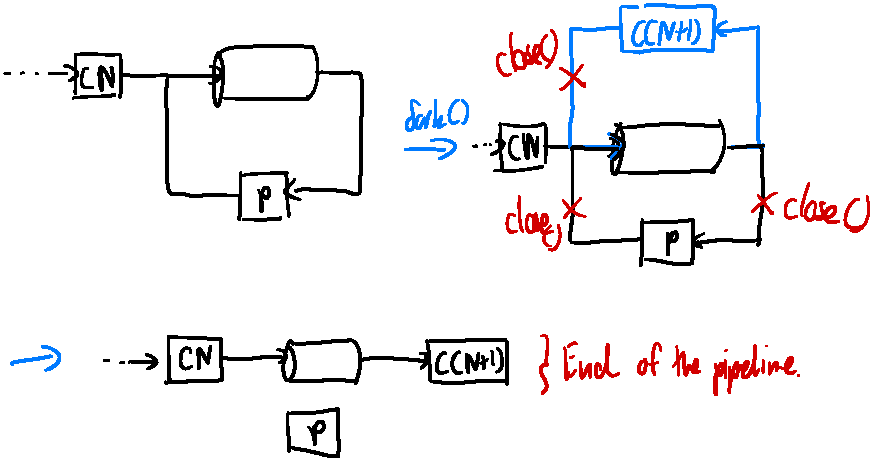
\includegraphics{task1qc2}
\caption{An illustration of the \ul{end} pattern used to
construct an arbitrary pipeline.}
\label{end_pipeline}
\end{figure}

For question (c), a new variant was created called
\texttt{execute\_pipeline()}. As input, it takes in a
\texttt{NULL}-terminated array of programs (including there
arguments).

The function constructs an arbitrary \ul{pipeline} which allows
every program to communicate with the next program. This is
achieved through the patterns illustrated in figures
\ref{gen_pipeline} and \ref{end_pipeline}.

\lstinputlisting[caption={The implementation of the described
mechanism for constructing a pipeline.},language=C,
firstline=22, lastline=79]{src/task1/qc.c}

In particular there are three distinct patterns which the
algorithm has to perform. These are labelled as \ul{start},
\ul{middle} (illustrated in figure \ref{gen_pipeline}) and
\ul{end} (illustrated in figure \ref{end_pipeline}). In
particular the middle step is repeated until the end is reached.

For the actual implementation the middle pattern is augmented
with \texttt{if}-statements to cater for the start and end
patterns.

\textit{Note:} There is no need to know the length of the
pipeline. This is because the only four file descriptors which
the parent process has awareness of at any one point in time
during the construction of a pipeline, are the file
descriptors associated with the previous and current pipe.

\lstinputlisting[caption={\texttt{waitpid()} being called in the
parent for every forked process.},language=C, firstline=80,
lastline=83]{src/task1/qd.c}

For question (d), an \texttt{options} parameter was added to the
previous function and a call to \texttt{waitpid()} is made for
every forked process (see the above listing).

\vspace{10pt}

\begin{figure}[H]
\centering
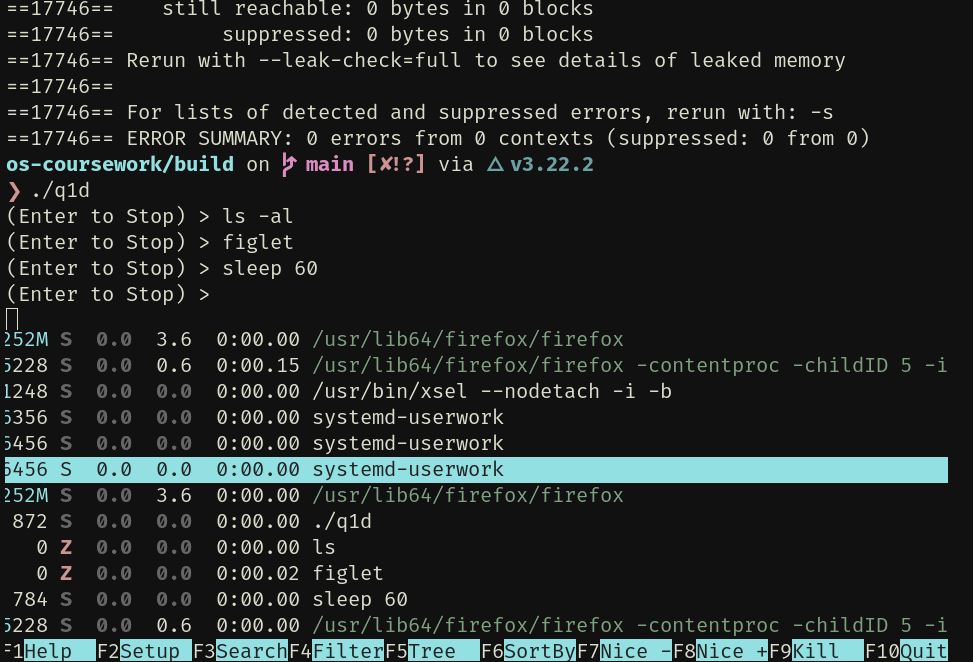
\includegraphics[width=12cm]{zombies}
\caption{A screenshot of zombie processes (in \texttt{htop})
present because the function waits only for the last process.}
\label{zombies}
\end{figure}

The function blocks for every process to ensure no zombie
processes are present. Figure \ref{zombies} demonstrates a
version of the question where the function blocks only for the
last process.

\newpage

\lstinputlisting[caption={Redirecting pipeline
input.},language=C, firstline=95, lastline=99]{src/task1/qe.c}

\lstinputlisting[caption={Redirecting pipeline
output.},language=C, firstline=123, lastline=129]{src/task1/qe.c}

For question (e), a simple addition of three extra parameters
and two \texttt{if}-statements in the start and end stages
suffice to redirect the input and the output of the pipe. The
third parameter is a flag used to choose between appending to a
file or truncating a file.

\subsubsection{Design of Task 2}

\lstinputlisting[caption={Code structures for supporting builtin
commands.}, language=C, firstline=71,
lastline=81]{src/task2/qab.c}

For question (a), what needs to be implemented is laid out
clearly in the question. Specifically, the creation of an array
for holding function pointers and function names together. 

\lstinputlisting[caption={\texttt{for}-loop to check if the
command is a builtin.}, language=C, firstline=91,
lastline=95]{src/task2/qab.c}

A linear search is performed every time before trying to execute
an external process to check if the specified command is a
builtin.

For question (b) a number of builtin functions had to be
implemented.

\texttt{sh\_exit()} is the simplest of the functions simply
calling the \texttt{exit()} function from \texttt{stdlib.h}.

\textit{Note:} In \textit{Task 3} and \textit{Task 4}
\texttt{sh\_exit()} was changed. These changes were made to
ensure proper termination (i.e. adequate relinquishing of
allocated resources).

\lstinputlisting[caption={The \texttt{\#define}s for
\texttt{sh\_ver()}.}, language=C, firstline=18,
lastline=22]{src/task2/qab.c}

\texttt{sh\_ver()} prints a formatted string to \texttt{stdout}
containing the author's name, version and a small message. The
author's name, version and message are all \texttt{\#define}s.

\lstinputlisting[caption={The declaration of the global
\texttt{cwd}.},language=C, firstline=10,
lastline=16]{src/task2/qab.c}

\newpage

\lstinputlisting[caption={Initialising
\texttt{cwd}.},language=C, firstline=114,
lastline=117]{src/task2/qab.c}

\texttt{sh\_cwd()} prints the contents of the global variable
\texttt{cwd} to \texttt{stdout}. \texttt{cwd} is a character
array with a length of \texttt{PATH\_MAX}, which is a definition
found in \texttt{linux/limits.h} on Linux. If the OS is not
Linux, the limit will be set to 4096 characters. Moreover, the
global has to be initialised at the start of the shell.

\texttt{sh\_cd()} uses \texttt{chdir()} to change the current
directory of the shell to the first argument provided to
\texttt{cd} or to the home directory of the current user if no
argument is provided. Naturally, \texttt{sh\_cd()} will have to
update \texttt{cwd} every time since the directory might change.

\subsubsection{Design of Task 3 and 4}

\begin{figure}[H]
\centering
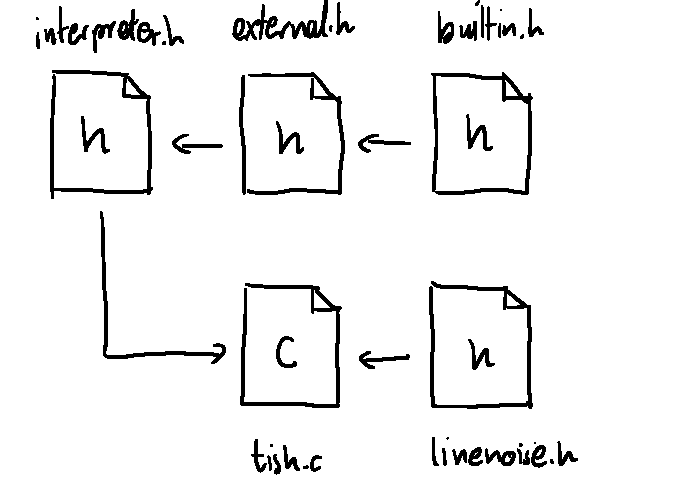
\includegraphics{task3arch}
\caption{An illustration of how the files used for \textit{Task
3} and \textit{Task 4} are linked (through \texttt{\#include}).}
\end{figure}

The design of these tasks has been merged into one.
Particularly, there are five main \texttt{.c} files.
\texttt{external.c} contains the functions written for
\textit{Task 1} and \texttt{builtin.c} contains the functions
written for \textit{Task 2}. \texttt{interpreter.c} is the file
where all the new functionality is present. Specifically, it
contains, the tokeniser, syntactic checker and translator.

Moreover, it also contains a simple \texttt{execute()} function
which interacts with the components in \texttt{external.c} and
\texttt{builtin.c} through header files.

\texttt{linenoise.c} is the suggest line editing library, which
allows for the easy creation of prompts and command line user
interfaces. The repository of the original author can be found
at: \url{https://github.com/antirez/linenoise}.

\texttt{tish.c} is the source file which brings all of these
components together to create a functional shell named `Tiny
Shell' (\texttt{tish}).

\begin{figure}[H]
\centering
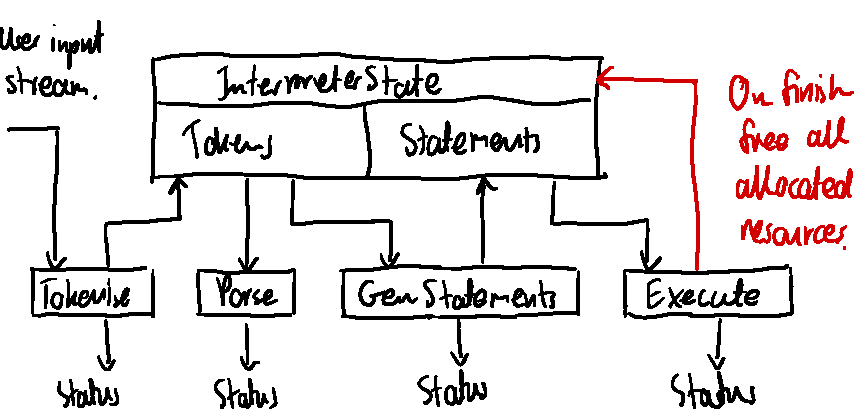
\includegraphics{interpreter-arch}
\caption{An illustration of how the interpreter is structured
and how it processes user input lines.}
\end{figure}

\lstinputlisting[caption={The \texttt{InterpreterState}
structure.},language=C,firstline=53,
lastline=63]{src/task3and4/interpreter.c}

In the interpreter there is one static global structure which is
used throughout all of the components of the interpreter. These
components/functions are the following: \texttt{tokenise()},
\texttt{parse()}, \texttt{genStatements()} and
\texttt{execute()}. There is one exposed function in the file
\texttt{interpret()} and it is called in \texttt{tish.c}.

\begin{figure}[H]
\centering
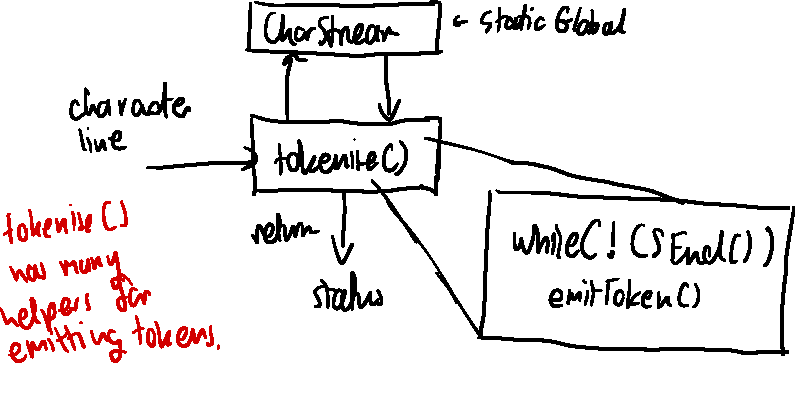
\includegraphics{tokeniser}
\caption{A simple illustration of how the tokeniser works.}
\end{figure}

\lstinputlisting[caption={The \texttt{CharStream}
structure.},language=C, firstline=16,
lastline=20]{src/task3and4/interpreter.c}

The \texttt{tokenise()} function makes use of a static global
called \texttt{CharStream}. This allows the tokeniser to
traverse a character array without losing state across different
function calls. It also makes the code cleaner.

\newpage

\lstinputlisting[caption={The section in \texttt{emitString()}
which handles escaping.},language=C, firstline=352,
lastline=364]{src/task3and4/interpreter.c}

The most important functions in the tokeniser are the emitters.
They basically emit a token which can later be used to check if
the user input is syntactically correct. Emitted tokens are
stored in the interpreter state. Escaping of characters is
performed in \texttt{emitString()}.

\begin{figure}[H]
\centering
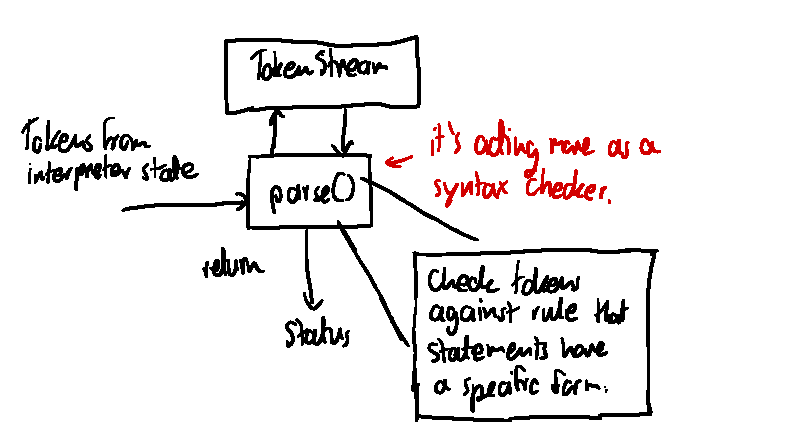
\includegraphics{parser}
\caption{A simple illustration of how the parser works.}
\end{figure}

\newpage

\lstinputlisting[caption={The \texttt{TokenStream}
structure.},language=C,firstline=37,
lastline=41]{src/task3and4/interpreter.c}

\texttt{parse()} initialises the \texttt{TokenStream} and checks
if the syntax of the tokens is correct. It also counts the
number of statements in single input.

\textit{Note:} Multiple statements in a single input have to
be separated by a semicolon (\texttt{;}).

The general form of a statement is:

\begin{verbatim}
pipeline := <redirect_cmd> | <pipeline> "|" <redirect_cmd>
redirect_cmd := <cmd>
              | <redirect_cmd> "<" <str>
              | <redirect_cmd> ">" <str>
              | <redirect_cmd> ">>" <str> 
cmd := str | <cmd> str
str := (contiguous string of characters not delimited
        by space or in double quotes)
\end{verbatim}

\textit{Note:} Characters such as \texttt{\textless},
\texttt{\textgreater}, \texttt{{\textgreater}{\textgreater}} are
optional. For example there is no need for input or/and output
redirection. Nevertheless, if for example, a
\texttt{\textgreater} is present it must be followed by an
\texttt{infile}.

If a collection of tokens cannot fit into the above production
rules, the parser will print an error and clean any allocated
resources.

After checking that the tokens are syntactically correct, the
\texttt{genStatements()} function can assume certain things
about structure of the tokens. The \texttt{genStatements()}
function does two main things. It counts the number of commands
in a pipeline and the number of strings (or arguments) per
command. This is done for every statement.

Having this information allows the function to allocate the
exact amount of memory required for the statements which are
then populated accordingly.

\textit{Note:} The process of counting, allocating and
populating are all done simultaneously throughout the code. This
is because it is more convenient for certain tasks to be done
when the information is directly available.

\newpage

\lstinputlisting[caption={Code for handling different return
codes.},language=C,firstline=832,
lastline=838]{src/task3and4/interpreter.c}

The \texttt{execute()} function has two parts. The first part
checks if the command is a builtin. If the command is a builtin
\texttt{execute()} will call the respective builtin function.
Otherwise, it will try to execute an external program.

\textit{Note:} There are two scenarios when -2, which is
defined as \texttt{EXIT\_SHELL}, is returned. First, when the
\texttt{exit()} builtin is called or second, when a forked
process fails. The latter case is special because it avoids the
possibility of having two concurrent shell processes where the
forked shell spins because its \texttt{stdin} is bound to a
pipe.

\lstinputlisting[caption={The \texttt{interpret()} function,
calls and handles each of the functions described
above.},language=C, firstline=871,
lastline=889]{src/task3and4/interpreter.c}

\newpage

The final function is \texttt{interpret()} and it collects all
of these functions together into one function which is called in
\texttt{tish.c}. Specifically, in \texttt{tish.c} there is an
event loop which waits for user input and then passes the user
input to \texttt{interpret()} and the process repeats until the
user decides to exit.

\section{Testing Methodology}

\subsection{Testing for Task 1}

\begin{figure}[H]
\centering
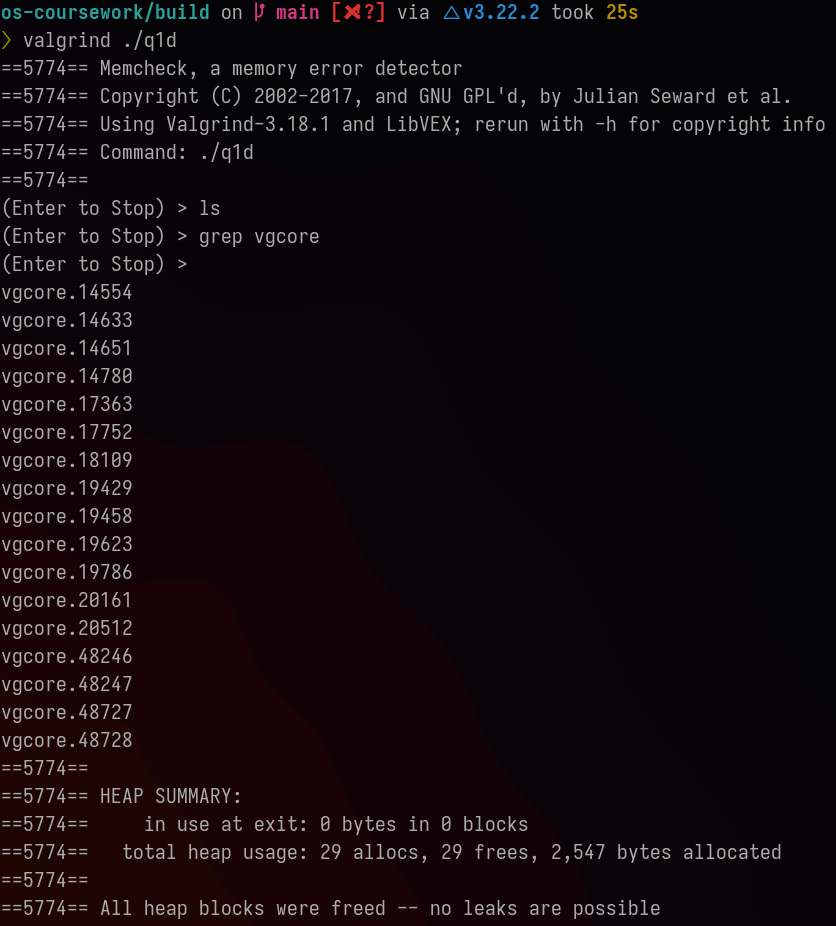
\includegraphics[width=11cm]{q1d-test}
\caption{A screenshot of the \texttt{q1d} executable running
under \texttt{valgrind}.}
\end{figure}

For testing, all functions developed in \textit{Task 1} were
isolated in there own file, with a simple main function.

The main function contains a simple prompt which allows for user
input. Commands were entered and the output was noted and
compared to the expected behaviour.

Moreover, \texttt{valgrind} was used to make sure that no memory
was being leaked and no errors were being report. Also, all
compiler warnings were enabled (see the \texttt{CMakeLists.txt}
file).

\textit{Note:} To properly test for blocking, a command like
\texttt{sleep 10} was used (see figure \ref{zombies}). Moreover,
testing for question (e) was done with hard coded file names
(see functions \texttt{test1()} and \texttt{test2()}
in \texttt{src/task1/qe.c}).

\subsection{Testing for Task 2}

\begin{figure}[H]
\centering
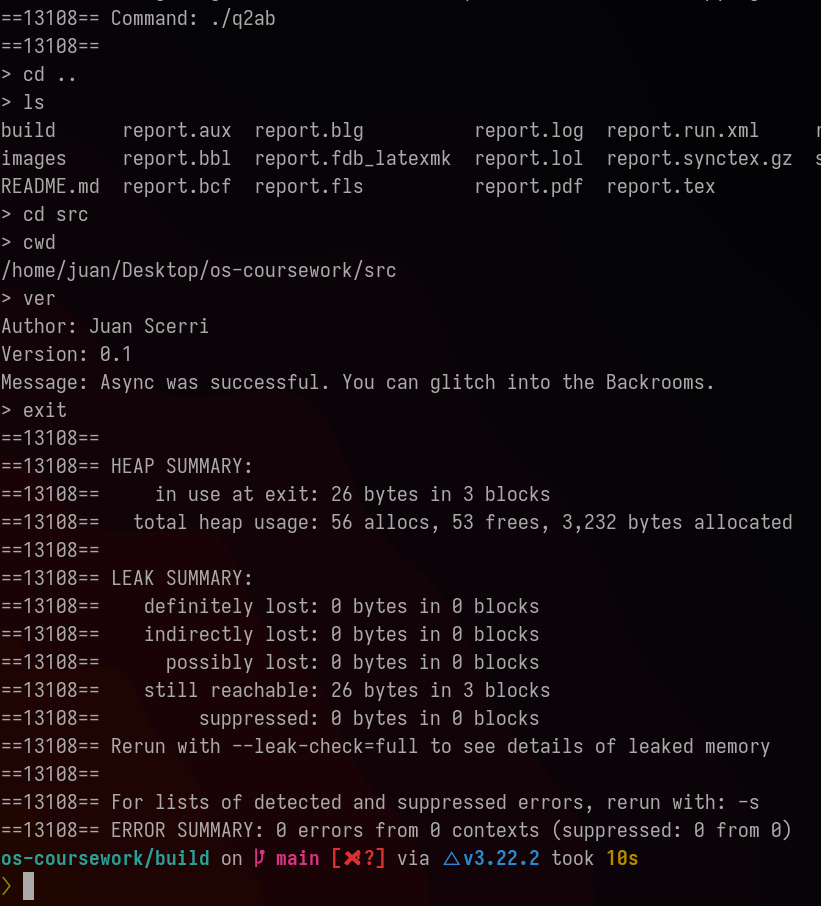
\includegraphics[width=12cm]{q2ab-test}
\caption{A screenshot of the \texttt{q2ab} executable running
under \texttt{valgrind}.}
\end{figure}

Testing for \textit{Task 2} was performed using a similar method
to \textit{Task 1}. An executable is generated which can be used
to test user input.

\textit{Note:} The implementation of \texttt{exit} in this task
leaks memory because it is using \texttt{exit()} without freeing
any potentially allocated data. This has been addressed in the
actual shell.

\subsection{Testing for Task 3}\label{testing-task3}

Testing for \textit{Task 3} is a bit more complicated because it
requires a lot of debug output to ensure that tokenisation,
parsing and translation (into statements) are being done
correctly.

\lstinputlisting[caption={Comment indicating the usage of
\texttt{\#define DEBUG}.},language=C, firstline=8,
lastline=10]{src/task3and4/interpreter.c}

% \lstinputlisting[caption={Usage of the \texttt{DEBUG} definition
% for debugging.},language=C, firstline=516,
% lastline=518]{src/task3and4/interpreter.c}

\begin{figure}[H]
\centering
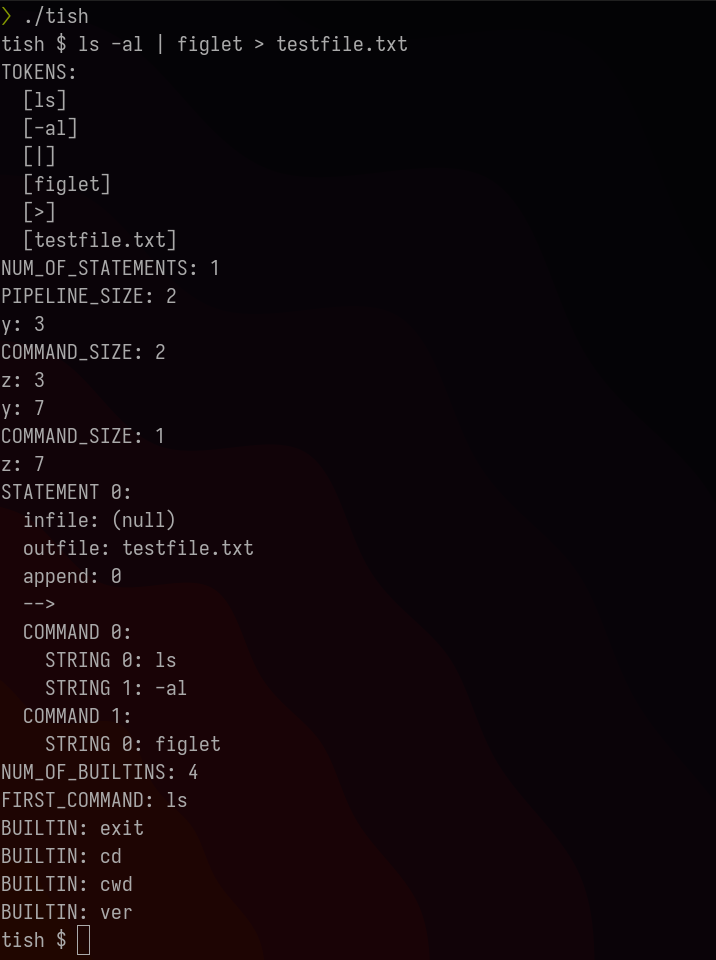
\includegraphics[width=10cm]{task3and4-test}
\caption{A screenshot of the \texttt{tish} executable running
with \texttt{DEBUG} defined.}
\end{figure}

To do this, a number of function calls to
\texttt{fprintf(stderr, ...)} are littered throughout the code.
They can be activated by defining \texttt{DEBUG} in the
\texttt{interpreter.c} source file and recompiling.

\newpage

\lstinputlisting[caption={The \texttt{tests.txt} file.}]{src/task3and4/tests.txt}

A list of test inputs can be found at
\texttt{src/task3and4/tests.txt}. There are eleven test inputs
and they are all identified as being either syntactically valid
or invalid.

\section{Issues \& Bugs}

\subsection{Issues}

There are a number of issues both with regards to the design of
the code and the functionality of the shell.

\subsubsection{Design Issues}

\begin{itemize}
\item
  The way in which the shell exits could be improved through the
  use of an exit handler.
\item
  The current implementation of \texttt{tish}, especially the
  interpreter relies heavily on heap-allocated memory. It would
  be beneficial if heap-allocations are reduced both for
  performance and code readability, as often times
  control flow is obscured because of constant validation and
  error checking.
\item
  The main data structures in use are stored as static (or
  scoped) global variables. It would be better if these
  structures are created on the stack frame of the main function
  and then passed by reference to the functions which require
  them. It would also improve the readability of the code.
\end{itemize}

\subsubsection{Functional Issues}

\begin{itemize}
\item
  The current shell does not conform to a \texttt{bash}-like
  syntax. So, improving compatibility with already existing
  shells would be beneficial.
\end{itemize}

\subsection{Bugs}

No undefined behaviour or bugs in the final binary (i.e.
\texttt{tish}) have been found.

Both reasonable and extreme examples of user input were used to
test the reliability of the shell and the code. The reasonable
examples used were those provided in
\texttt{tiny\_shell\_examples.pdf}. The extreme examples used
were those described in \ref{testing-task3}.

As mentioned throughout the document there were some minor
issues (e.g. memory leaks, zombies etc.) which were present in
\textbf{earlier} versions of the code. However, these are
\textbf{not} present in the final binary (i.e. \texttt{tish}).

\end{document}
